\documentclass[aspectratio=169,11pt]{beamer}

\usepackage[T1]{fontenc}
\usepackage[utf8]{inputenc}
\usepackage[brazilian]{babel}
\usepackage{lmodern}
\usepackage{graphicx}
\usepackage{booktabs}
\usepackage{amsmath}
\usepackage{pgfplots}
\pgfplotsset{compat=1.18}
\usepackage{hyperref}
\usepackage{multicol}
\usepackage{tikz}

% -----------------------------------------------------------------------------
% Identidade visual
% -----------------------------------------------------------------------------
\definecolor{RoxoPrincipal}{HTML}{4D4057}
\definecolor{RoxoSecundario}{HTML}{75657F}
\definecolor{MalvaDestaque}{HTML}{9A6F86}
\definecolor{LavandaClaro}{HTML}{F1EDF3}
\definecolor{LavandaLinha}{HTML}{D8CFDD}
\definecolor{CinzaTexto}{HTML}{413C43}

\usetheme{default}
\useinnertheme{rounded}
\setbeamertemplate{navigation symbols}{}

\setbeamercolor{normal text}{fg=CinzaTexto,bg=white}
\setbeamercolor{structure}{fg=RoxoPrincipal}
\setbeamercolor{title}{fg=white}
\setbeamercolor{subtitle}{fg=white}
\setbeamercolor{author}{fg=white}
\setbeamercolor{institute}{fg=white!90}
\setbeamercolor{date}{fg=white!80}
\setbeamercolor{frametitle}{fg=white,bg=RoxoPrincipal}
\setbeamercolor{block title}{fg=white,bg=RoxoSecundario}
\setbeamercolor{block body}{fg=CinzaTexto,bg=LavandaClaro}
\setbeamercolor{block title alerted}{fg=white,bg=MalvaDestaque}
\setbeamercolor{block body alerted}{fg=CinzaTexto,bg=LavandaClaro}
\setbeamercolor{alerted text}{fg=MalvaDestaque}
\setbeamercolor{footline}{fg=RoxoPrincipal,bg=white}
\setbeamercolor{footline line}{bg=LavandaLinha}

\setbeamerfont{title}{size=\LARGE,series=\bfseries}
\setbeamerfont{subtitle}{size=\large}
\setbeamerfont{frametitle}{size=\large,series=\bfseries}
\setbeamerfont{footline}{size=\scriptsize}

% Logo da UFPE com uma base clara para contraste.
\newcommand{\marcaInstitucional}[1]{%
  \begin{tikzpicture}[baseline=(marca.base)]
    \node[fill=white,rounded corners=2pt,inner sep=2.2pt] (marca) {%
      
\includegraphics[height=#1]{logo_ufpe.png}%
    };
  \end{tikzpicture}%
}

% Cabeçalho roxo com a marca institucional em todos os slides de conteúdo.
\setbeamertemplate{frametitle}{%
  \nointerlineskip
  \begin{beamercolorbox}[
    wd=\paperwidth,ht=3.4ex,dp=1.45ex,leftskip=0.58cm,rightskip=1.75cm
  ]{frametitle}%
    \usebeamerfont{frametitle}\insertframetitle
  \end{beamercolorbox}%
  \begin{tikzpicture}[remember picture,overlay]
    \node[anchor=north east,fill=white,rounded corners=2pt,inner sep=1.2pt]
      at ([xshift=-0.32cm,yshift=-0.16cm]current page.north east)
      {
\includegraphics[height=0.52cm]{logo_ufpe.png}};
  \end{tikzpicture}%
}

% Rodapé leve, com seção atual e paginação em formato de cápsula.
\setbeamertemplate{footline}{%
  \leavevmode%
  \vbox{%
    \begin{beamercolorbox}[wd=\paperwidth,ht=0.22ex,dp=0ex]{footline line}
    \end{beamercolorbox}%
    \hbox{%
      \begin{beamercolorbox}[wd=.28\paperwidth,ht=3.0ex,dp=1.15ex,leftskip=0.55cm]{footline}
        \usebeamerfont{footline}\insertshortauthor
      \end{beamercolorbox}%
      \begin{beamercolorbox}[wd=.52\paperwidth,ht=3.0ex,dp=1.15ex,center]{footline}
        \usebeamerfont{footline}\insertsectionhead
      \end{beamercolorbox}%
      \begin{beamercolorbox}[wd=.20\paperwidth,ht=3.0ex,dp=0.65ex,rightskip=0.45cm plus 1fil]{footline}
        \tikz[baseline=-0.65ex]{%
          \node[fill=RoxoPrincipal,text=white,rounded corners=5pt,
            inner xsep=7pt,inner ysep=2.3pt] {%
            \usebeamerfont{footline}\insertframenumber\,/\,\inserttotalframenumber
          };
        }%
      \end{beamercolorbox}%
    }%
  }%
  \vskip0pt%
}

% -----------------------------------------------------------------------------
% Informações editáveis da apresentação
% -----------------------------------------------------------------------------
\newcommand{\telefone}{(81) 98538-4702}
\newcommand{\email}{Romadeoliveira@hotmail.com}
\newcommand{\linkedin}{linkedin.com/in/romariojonas-veloso-427373175}
\newcommand{\portfolio}{romariojonas.com}
\newcommand{\lattes}{lattes.cnpq.br/7040983804231610}

\title[Filtro ativo de segunda ordem]{Filtro Ativo Passa-Baixa de Segunda Ordem}
\subtitle{Resposta em frequência e transitória de duas configurações com amplificador operacional}
\author[Romário J. O. Veloso]{Romário J. O. Veloso}
\institute{Bacharelando em Engenharia Eletrônica\\
Universidade Federal de Pernambuco -- UFPE\\
Centro de Tecnologia e Geociências -- CTG\\
Departamento de Eletrônica e Sistemas -- DES}
\date{Prática 3 -- Circuitos Elétricos 2 -- 2026.2}

\pgfplotsset{
  grafico/.style={
    width=\linewidth,
    height=0.49\textheight,
    grid=both,
    major grid style={LavandaLinha},
    minor grid style={LavandaClaro},
    tick label style={font=\scriptsize},
    label style={font=\scriptsize},
    legend style={font=\scriptsize,draw=none,fill=white},
    scaled ticks=false,
  }
}

\begin{document}

{
\setbeamercolor{background canvas}{bg=RoxoPrincipal}
\setbeamertemplate{footline}{}
\begin{frame}[plain]
  \begin{center}
    \vspace{0.06cm}
    \marcaInstitucional{1.30cm}\par
    \vspace{0.28cm}
    {\usebeamerfont{title}\color{white}\inserttitle\par}
    \vspace{0.18cm}
    {\usebeamerfont{subtitle}\color{white!82}\insertsubtitle\par}
    \vspace{0.26cm}
    {\color{MalvaDestaque}\rule{0.22\textwidth}{2pt}}\par
    \vspace{0.26cm}
    {\usebeamerfont{author}\color{white}\insertauthor\par}
    \vspace{0.10cm}
    {\usebeamerfont{institute}\color{white!84}\insertinstitute\par}
    \vfill
    {\color{white!72}\small\insertdate\quad\textbullet\quad Recife -- Pernambuco}
  \end{center}
\end{frame}
}

\begin{frame}{Sumário}
  \tableofcontents[hideallsubsections]
\end{frame}


\section{Introdução}
\begin{frame}{Contexto da prática}
  \begin{block}{Problema investigado}
    Como a troca dos valores de dois resistores altera o ganho, o amortecimento e
    a resposta transitória de um filtro ativo passa-baixa de segunda ordem?
  \end{block}

  \begin{columns}[T,onlytextwidth]
    \begin{column}{0.48\textwidth}
      \textbf{Regime permanente senoidal}
      \begin{itemize}
        \item magnitude e fase de $H(j\omega)$;
        \item ganho em baixas frequências;
        \item frequência de corte de $-3\,\mathrm{dB}$;
        \item possível pico de ressonância.
      \end{itemize}
    \end{column}
    \begin{column}{0.48\textwidth}
      \textbf{Regime transitório}
      \begin{itemize}
        \item resposta a uma entrada em degrau;
        \item valor final da tensão de saída;
        \item tempos $t_{10}$ e $t_{90}$;
        \item resposta monótona ou oscilatória.
      \end{itemize}
    \end{column}
  \end{columns}
\end{frame}

\begin{frame}{Objetivos}
  \begin{block}{Objetivo geral}
    Analisar o comportamento permanente e transitório de duas configurações de
    um circuito de segunda ordem com amplificador operacional, comparando teoria,
    simulação e medições em laboratório.
  \end{block}

  \begin{itemize}
    \item Deduzir a função de transferência $H(s)=V_o(s)/V_i(s)$.
    \item Calcular os polos e os diagramas de Bode dos dois circuitos.
    \item Determinar a resposta ao degrau e os tempos para atingir 10\% e 90\% do valor final.
    \item Validar as respostas em frequência no LTspice.
    \item Comparar os resultados com as amplitudes e os transitórios registrados em bancada.
  \end{itemize}
\end{frame}

\begin{frame}{Metodologia de validação}
  \small
  \begin{columns}[T,onlytextwidth]
    \begin{column}{0.31\textwidth}
      \begin{block}{1. Análise teórica}
        \begin{itemize}
          \item equações nodais e modelo ideal do ampop;
          \item resolução simbólica com SymPy;
          \item Bode entre $0{,}01$ e $10^5\,\mathrm{Hz}$;
          \item transformada inversa de Laplace.
        \end{itemize}
      \end{block}
    \end{column}
    \begin{column}{0.31\textwidth}
      \begin{block}{2. Simulação}
        \begin{itemize}
          \item duas configurações no LTspice;
          \item alimentação de $\pm10\,\mathrm{V}$;
          \item análise AC com entrada unitária;
          \item excitações transitórias de $0{,}8$ e $5\,\mathrm{V}$.
        \end{itemize}
      \end{block}
    \end{column}
    \begin{column}{0.31\textwidth}
      \begin{block}{3. Ensaio em bancada}
        \begin{itemize}
          \item conferência dos componentes;
          \item montagem em protoboard;
          \item gerador e osciloscópio de dois canais;
          \item medição de amplitudes, corte e tempos.
        \end{itemize}
      \end{block}
    \end{column}
  \end{columns}

  \begin{alertblock}{Grandezas de comparação}
    \centering
    $|H(j\omega)|=V_o/V_i$
    \qquad
    $V_o(f_c)=V_o(0)/\sqrt{2}$
    \qquad
    $t_r=t_{90}-t_{10}$.
  \end{alertblock}
\end{frame}

\begin{frame}{Circuito ativo e configurações estudadas}
  \begin{columns}[c,onlytextwidth]
    \begin{column}{0.54\textwidth}
      \centering
      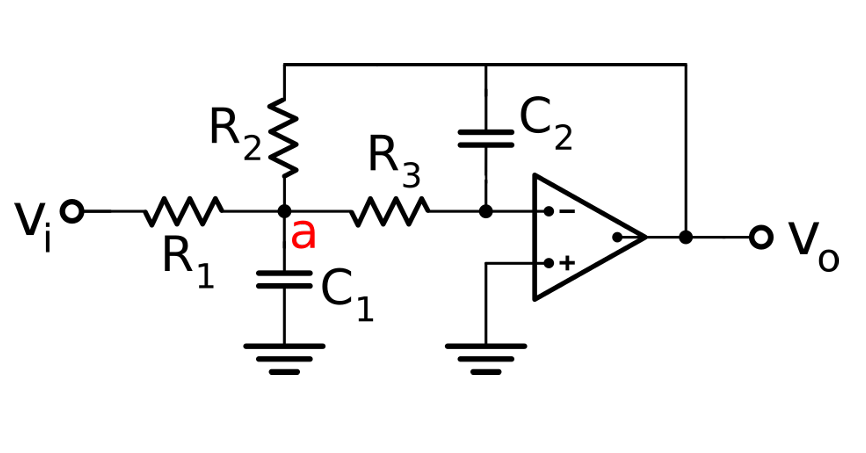
\includegraphics[width=\linewidth]{slides/img/circuito_passabaixa.png}

      \vspace{0.14cm}
      \scriptsize Topologia passa-baixa de realimentação múltipla.
    \end{column}
    \begin{column}{0.43\textwidth}
      \small
      \begin{block}{Componentes comuns}
        $C_1=100\,\mathrm{nF}$, $C_2=10\,\mathrm{nF}$\\
        $R_2=470\,\mathrm{k}\Omega$; alimentação: $\pm10\,\mathrm{V}$.
      \end{block}

      \begin{tabular}{lcc}
        \toprule
        & Circuito 1 & Circuito 2 \\
        \midrule
        $R_1$ & $47\,\mathrm{k}\Omega$ & $470\,\mathrm{k}\Omega$ \\
        $R_3$ & $470\,\mathrm{k}\Omega$ & $47\,\mathrm{k}\Omega$ \\
        \bottomrule
      \end{tabular}

      \begin{alertblock}{Alteração investigada}
        A troca entre $R_1$ e $R_3$ modifica o ganho e a posição dos polos,
        preservando a topologia.
      \end{alertblock}
    \end{column}
  \end{columns}
\end{frame}


\section{Análise teórica}
\begin{frame}{Modelagem no domínio de Laplace}
  \small
  \begin{columns}[T,onlytextwidth]
    \begin{column}{0.44\textwidth}
      \begin{block}{Equações nodais}
        \[
          C_1sV_a+\frac{V_a}{R_3}+\frac{V_a-V_o}{R_2}
          +\frac{V_a-V_i}{R_1}=0
        \]
        \[
          V_a=-C_2R_3sV_o.
        \]
        No modelo ideal, $i^+=i^-=0$.
        Como $V_o=A(v^+-v^-)$ e $A\to\infty$, a realimentação impõe
        $v^-\approx v^+=0$: o terminal inversor está em terra virtual.
      \end{block}
    \end{column}
    \begin{column}{0.53\textwidth}
      \begin{alertblock}{Função de transferência}
        \[
          H(s)=\frac{-R_2}{a s^2+b s+R_1}
        \]
        \[
          a=C_1C_2R_1R_2R_3
        \]
        \[
          b=C_2(R_1R_2+R_1R_3+R_2R_3).
        \]
        Forma normalizada:
        \[
          H(s)=\frac{K\omega_n^2}{s^2+2\zeta\omega_n s+\omega_n^2},
          \qquad K=-\frac{R_2}{R_1}.
        \]
      \end{alertblock}
    \end{column}
  \end{columns}

  \vspace{0.08cm}
  \centering
  \alert{$\omega_n=\sqrt{R_1/a}$ \quad e \quad $\zeta=b/(2\sqrt{aR_1})$.}
\end{frame}

\begin{frame}{Funções de transferência e polos}
  \small
  \begin{columns}[T,onlytextwidth]
    \begin{column}{0.48\textwidth}
      \begin{block}{Circuito 1}
        \[
          H_1(s)=\frac{-470000}
          {10{,}3823s^2+2650{,}8s+47000}
        \]
        \[
          p_1\approx-19{,}17\,\mathrm{s}^{-1},\qquad
          p_2\approx-236{,}15\,\mathrm{s}^{-1}.
        \]
        \begin{itemize}
          \item $K_1=-10$; magnitude em DC: $20\,\mathrm{dB}$.
          \item $\omega_{n1}\approx67{,}28\,\mathrm{rad/s}$.
          \item $\zeta_1\approx1{,}897$: sobreamortecido.
          \item Resposta ao degrau monótona.
        \end{itemize}
      \end{block}
    \end{column}
    \begin{column}{0.48\textwidth}
      \begin{block}{Circuito 2}
        \[
          H_2(s)=\frac{-470000}
          {10{,}3823s^2+2650{,}8s+470000}
        \]
        \[
          p_{1,2}\approx-127{,}66\pm j170{,}21\,\mathrm{s}^{-1}.
        \]
        \begin{itemize}
          \item $K_2=-1$; magnitude em DC: $0\,\mathrm{dB}$.
          \item $\omega_{n2}\approx212{,}77\,\mathrm{rad/s}$.
          \item $\zeta_2=0{,}6$: subamortecido.
          \item Oscilação amortecida e sobressinal.
        \end{itemize}
      \end{block}
    \end{column}
  \end{columns}

  \vspace{0.12cm}
  \centering\scriptsize
  Polos obtidos de $\operatorname{den}H(s)=0$.
  As partes reais negativas garantem estabilidade e o decaimento dos termos transitórios.
\end{frame}

\begin{frame}{Resposta teórica em frequência}
  \begin{columns}[c,onlytextwidth]
    \begin{column}{0.48\textwidth}
      \centering
      \begin{tikzpicture}
        \begin{semilogxaxis}[
          grafico,width=0.96\linewidth,xmin=0.01,xmax=100000,ymin=-160,ymax=25,
          xlabel={Frequência (Hz)},ylabel={Magnitude (dB)},
          legend pos=south west
        ]
          \addplot[very thick,RoxoPrincipal] table[x=f,y=ganho1_db]{slides/dados/resposta_frequencia.dat};
          \addlegendentry{Circuito 1}
          \addplot[very thick,MalvaDestaque,dashed] table[x=f,y=ganho2_db]{slides/dados/resposta_frequencia.dat};
          \addlegendentry{Circuito 2}
        \end{semilogxaxis}
      \end{tikzpicture}
    \end{column}
    \begin{column}{0.48\textwidth}
      \centering
      \begin{tikzpicture}
        \begin{semilogxaxis}[
          grafico,xmin=0.01,xmax=100000,ymin=0,ymax=190,
          ytick={0,45,90,135,180},
          xlabel={Frequência (Hz)},ylabel={Fase (graus)}
        ]
          \addplot[very thick,RoxoPrincipal] table[x=f,y=fase1_deg]{slides/dados/resposta_frequencia.dat};
          \addplot[very thick,MalvaDestaque,dashed] table[x=f,y=fase2_deg]{slides/dados/resposta_frequencia.dat};
        \end{semilogxaxis}
      \end{tikzpicture}
    \end{column}
  \end{columns}

  \small
  \begin{block}{Leitura dos diagramas}
    Ambos os circuitos atenuam altas frequências a $-40\,\mathrm{dB}$ por década.
    O circuito 2 apresenta um pico suave próximo de $17{,}9\,\mathrm{Hz}$,
    com $|H|_{\max}\approx1{,}042$.
  \end{block}
  \centering\scriptsize
  Com $s=j2\pi f$: $M(f)=20\log_{10}|H(j2\pi f)|$ e $\phi(f)=\arg H(j2\pi f)$.
  A fase é apresentada no ramo de $180^\circ$ a $0^\circ$.
\end{frame}

\begin{frame}{Do degrau à resposta no tempo}
  \small
  \setlength{\abovedisplayskip}{4pt}
  \setlength{\belowdisplayskip}{4pt}
  Para $v_i(t)=A\,u(t)$ e condições iniciais nulas,
  $V_i(s)=A/s$ e $V_o(s)=H(s)A/s$.

  \begin{columns}[T,onlytextwidth]
    \begin{column}{0.48\textwidth}
      \begin{block}{Circuito 1: $A=0{,}8\,\mathrm{V}$}
        \[
          \begin{aligned}
            v_{o1}(t)\approx{}&-8
              +8{,}7068\,e^{-19{,}1698t}\\
              &-0{,}7068\,e^{-236{,}1494t}.
          \end{aligned}
        \]
        Resposta monótona: $v_{o1}(0)=0$ e
        $v_{o1}(\infty)=-8\,\mathrm{V}$.
      \end{block}
    \end{column}
    \begin{column}{0.48\textwidth}
      \begin{block}{Circuito 2: $A=5\,\mathrm{V}$}
        \[
          \begin{aligned}
            v_{o2}(t)\approx{}&-5+5e^{-127{,}6596t}\\
              &\!\!\times\bigl[\cos(170{,}2128t)\\
              &\quad+0{,}75\sin(170{,}2128t)\bigr].
          \end{aligned}
        \]
        Oscilação amortecida e sobressinal antes da convergência para $-5\,\mathrm{V}$.
      \end{block}
    \end{column}
  \end{columns}

  \begin{alertblock}{Valor final e estabilidade}
    Como os polos de $sV_o(s)$ têm parte real negativa,
    \[
      \lim_{t\to\infty}v_o(t)=\lim_{s\to0}sV_o(s)
      =A\,H(0)=-A\frac{R_2}{R_1}.
    \]
  \end{alertblock}
  \centering\scriptsize Inversa de Laplace para $t\geq0$, com $t$ em segundos e $v_o$ em volts.
\end{frame}

\begin{frame}{Resposta teórica ao degrau}
  \begin{columns}[T,onlytextwidth]
    \begin{column}{0.48\textwidth}
      \centering
      \textbf{Circuito 1: degrau de $0{,}8\,\mathrm{V}$}

      \begin{tikzpicture}
        \begin{axis}[
          grafico,height=0.43\textheight,
          xmin=0,xmax=500,ymin=-8.6,ymax=0.4,
          xlabel={Tempo (ms)},ylabel={$v_o(t)$ (V)}
        ]
          \addplot[very thick,RoxoPrincipal] table[x=t1_ms,y=saida1_v]{slides/dados/resposta_degrau.dat};
          \addplot[dashed,MalvaDestaque] coordinates {(0,-8) (500,-8)};
          \addplot[only marks,mark=*,MalvaDestaque] coordinates {(9.35,-0.8) (124.53,-7.2)};
        \end{axis}
      \end{tikzpicture}

      \small
      $v_o(\infty)=-8\,\mathrm{V}$\\
      $t_{10}\approx9{,}35\,\mathrm{ms}$; $t_{90}\approx124{,}53\,\mathrm{ms}$.
    \end{column}
    \begin{column}{0.48\textwidth}
      \centering
      \textbf{Circuito 2: degrau de $5\,\mathrm{V}$}

      \begin{tikzpicture}
        \begin{axis}[
          grafico,height=0.43\textheight,
          xmin=0,xmax=60,ymin=-5.8,ymax=0.3,
          xlabel={Tempo (ms)},ylabel={$v_o(t)$ (V)}
        ]
          \addplot[very thick,MalvaDestaque] table[x=t2_ms,y=saida2_v]{slides/dados/resposta_degrau.dat};
          \addplot[dashed,RoxoSecundario] coordinates {(0,-5) (60,-5)};
          \addplot[only marks,mark=*,RoxoPrincipal] coordinates {(2.33,-0.5) (11.05,-4.5)};
        \end{axis}
      \end{tikzpicture}

      \small
      $v_o(\infty)=-5\,\mathrm{V}$\\
      $t_{10}\approx2{,}33\,\mathrm{ms}$; $t_{90}\approx11{,}05\,\mathrm{ms}$.
    \end{column}
  \end{columns}

  \vspace{0.12cm}
  \centering\scriptsize
  Circuito 1: intervalo de $0$ a $0{,}5\,\mathrm{s}$.
  Circuito 2: detalhe dos primeiros $60\,\mathrm{ms}$.
  Os pontos indicam os níveis de 10\% e 90\% do valor final.
\end{frame}

\begin{frame}{Níveis de 10\% e 90\% da resposta}
  \small
  \setlength{\abovedisplayskip}{4pt}
  \setlength{\belowdisplayskip}{4pt}
  A partir do instante do degrau, buscam-se os níveis negativos da saída inversora:
  \[
    v_o(t_{10})=0{,}1\,v_o(\infty),
    \qquad
    v_o(t_{90})=0{,}9\,v_o(\infty).
  \]

  \begin{block}{Cálculo a partir da resposta analítica}
    No circuito 1, resolvem-se numericamente
    $v_{o1}(t_{10})=-0{,}8\,\mathrm{V}$ e
    $v_{o1}(t_{90})=-7{,}2\,\mathrm{V}$.
    No circuito 2, considera-se o primeiro cruzamento de cada nível.
  \end{block}

  {\centering
    \renewcommand{\arraystretch}{1.0}
    \begin{tabular}{lccccc}
      \toprule
      & $v_{10}$ (V) & $t_{10}$ (ms) & $v_{90}$ (V) & $t_{90}$ (ms) & $t_r$ (ms) \\
      \midrule
      Circuito 1 & $-0{,}8$ & $9{,}35$ & $-7{,}2$ & $124{,}53$ & $115{,}18$ \\
      Circuito 2 & $-0{,}5$ & $2{,}33$ & $-4{,}5$ & $11{,}05$ & $8{,}71$ \\
      \bottomrule
    \end{tabular}
    \par
  }

  \begin{alertblock}{Interpretação temporal}
    Com $t_r=t_{90}-t_{10}$, o circuito 2 completa a transição entre os dois níveis
    mais rapidamente, com oscilação amortecida.
  \end{alertblock}
  \centering\scriptsize
  Valores teóricos do modelo nominal; arredondamento aplicado ao final dos cálculos.
\end{frame}


\section{Validação}
\begin{frame}{Validação no LTspice: circuitos}
  \begin{columns}[T,onlytextwidth]
    \begin{column}{0.48\textwidth}
      \centering
      \textbf{Circuito 1}

      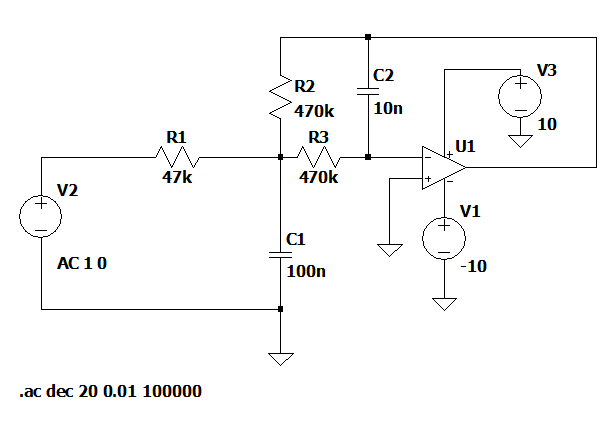
\includegraphics[width=\linewidth,height=0.47\textheight,keepaspectratio]{slides/img/ltspice_circuito_1.png}

      \small $R_1=47\,\mathrm{k}\Omega$, $R_3=470\,\mathrm{k}\Omega$.
    \end{column}
    \begin{column}{0.48\textwidth}
      \centering
      \textbf{Circuito 2}

      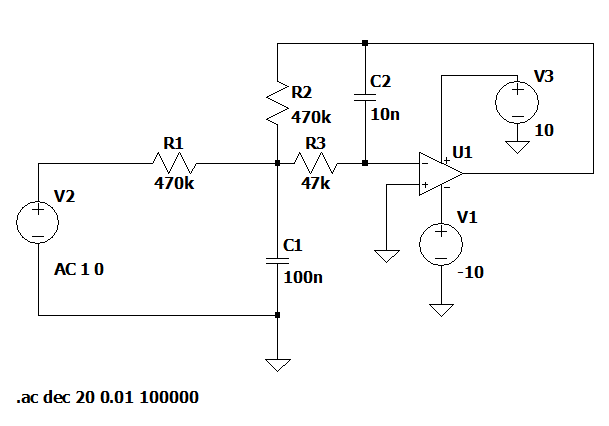
\includegraphics[width=\linewidth,height=0.47\textheight,keepaspectratio]{slides/img/ltspice_circuito_2.png}

      \small $R_1=470\,\mathrm{k}\Omega$, $R_3=47\,\mathrm{k}\Omega$.
    \end{column}
  \end{columns}

  \small
  \begin{block}{Configuração das simulações descritas no relatório}
    Análise AC: amplitude unitária, fase nula e varredura de $0{,}01$ a $10^5\,\mathrm{Hz}$.
    Alimentação do ampop: $\pm10\,\mathrm{V}$.
    Ensaios transitórios: onda quadrada de $0{,}8\,\mathrm{V}$ a $1\,\mathrm{Hz}$
    e de $5\,\mathrm{V}$ a $5\,\mathrm{Hz}$, respectivamente.
  \end{block}
\end{frame}

\begin{frame}{Validação no LTspice: resposta em frequência}
  \small
  \begin{columns}[T,onlytextwidth]
    \begin{column}{0.48\textwidth}
      \centering
      \textbf{Circuito 1}

      \vspace{0.06cm}
      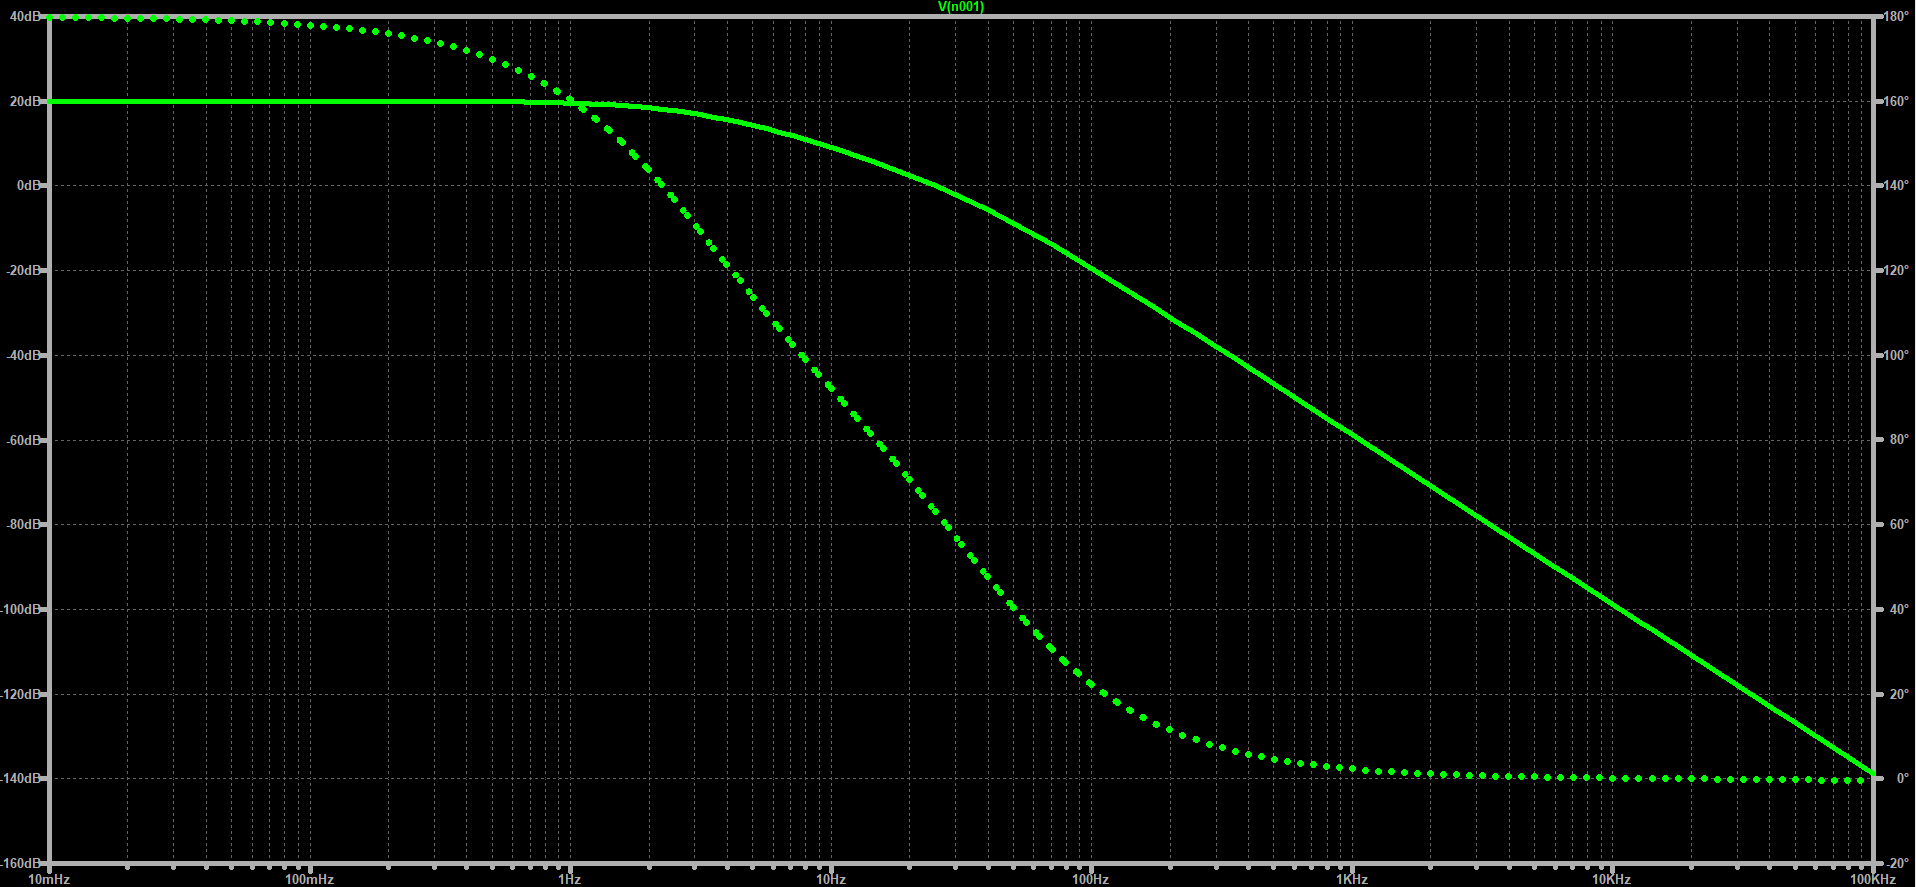
\includegraphics[width=\linewidth]{slides/img/ltspice_bode_1.png}

      \vspace{0.06cm}
      \small Ganho elevado em baixas frequências e atenuação progressiva.
    \end{column}
    \begin{column}{0.48\textwidth}
      \centering
      \textbf{Circuito 2}

      \vspace{0.06cm}
      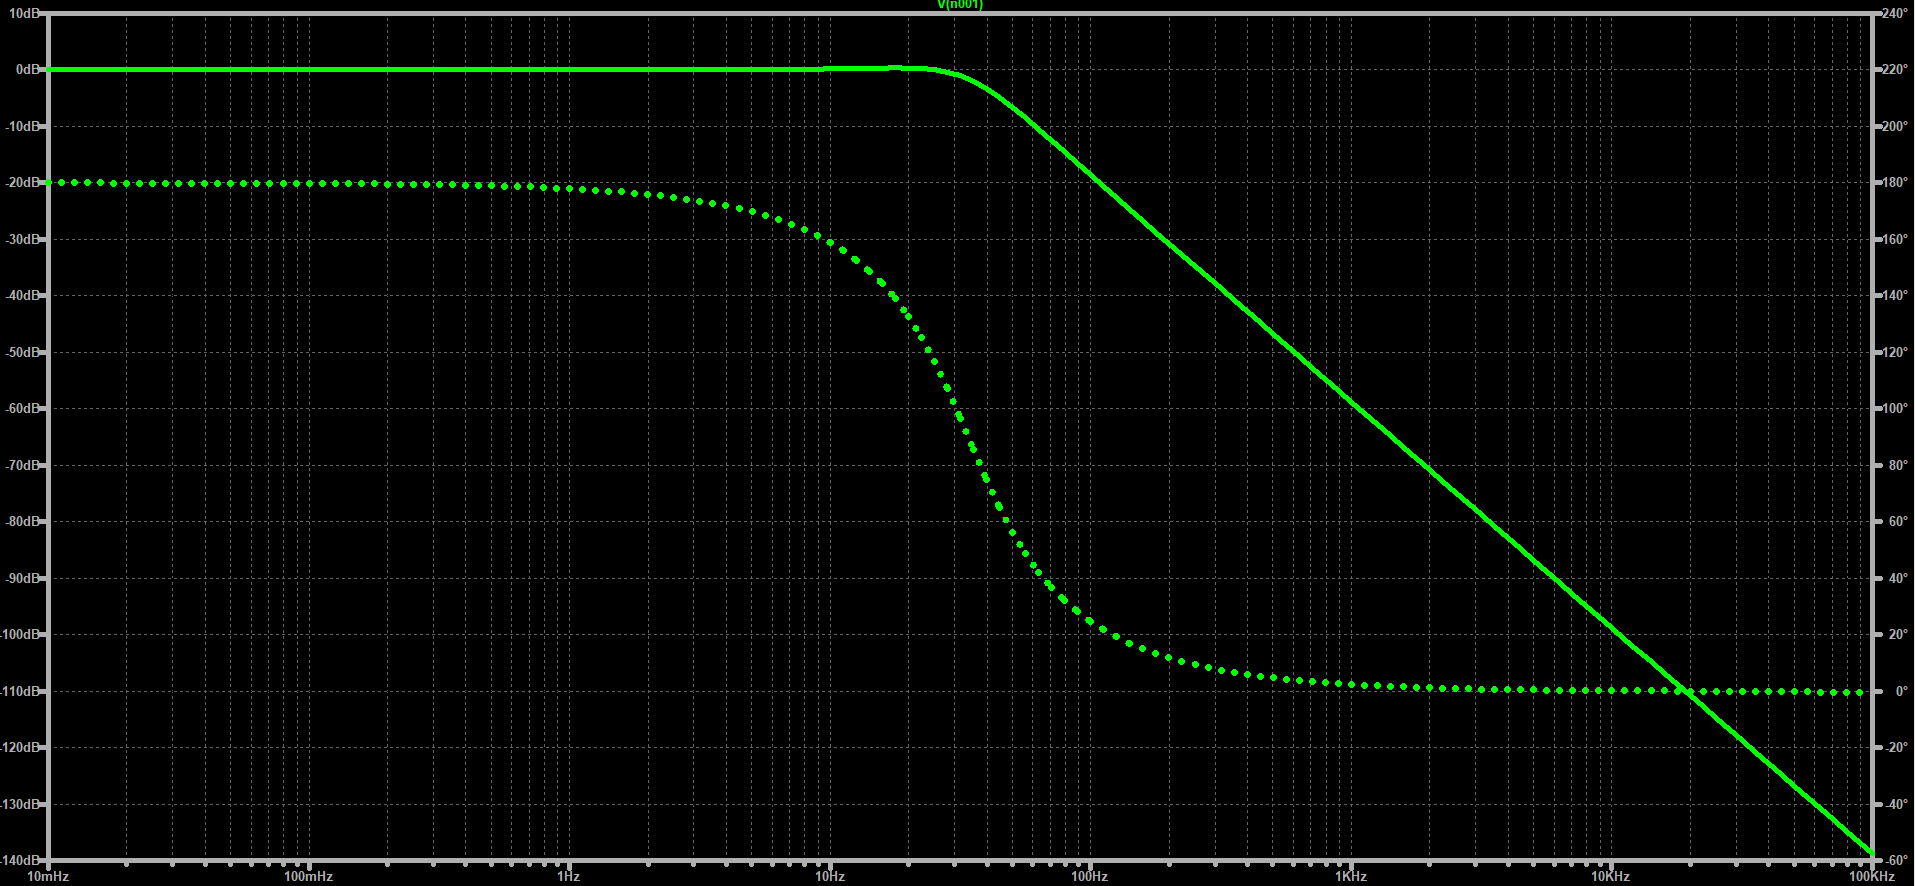
\includegraphics[width=\linewidth]{slides/img/ltspice_bode_2.png}

      \vspace{0.06cm}
      \small Ganho próximo da unidade, pequeno pico e transição mais acentuada.
    \end{column}
  \end{columns}

  \vspace{0.04cm}
  \begin{alertblock}{Comparação com o modelo}
    As curvas reproduzem a característica passa-baixa e o efeito da troca de
    resistores. A comparação é qualitativa: o relatório não apresenta erros
    numéricos da simulação.
  \end{alertblock}
  \centering\scriptsize Capturas originais da prática; magnitude e fase no mesmo painel.
\end{frame}

\begin{frame}{Montagem e conferência dos componentes}
  \begin{columns}[c,onlytextwidth]
    \begin{column}{0.46\textwidth}
      \centering
      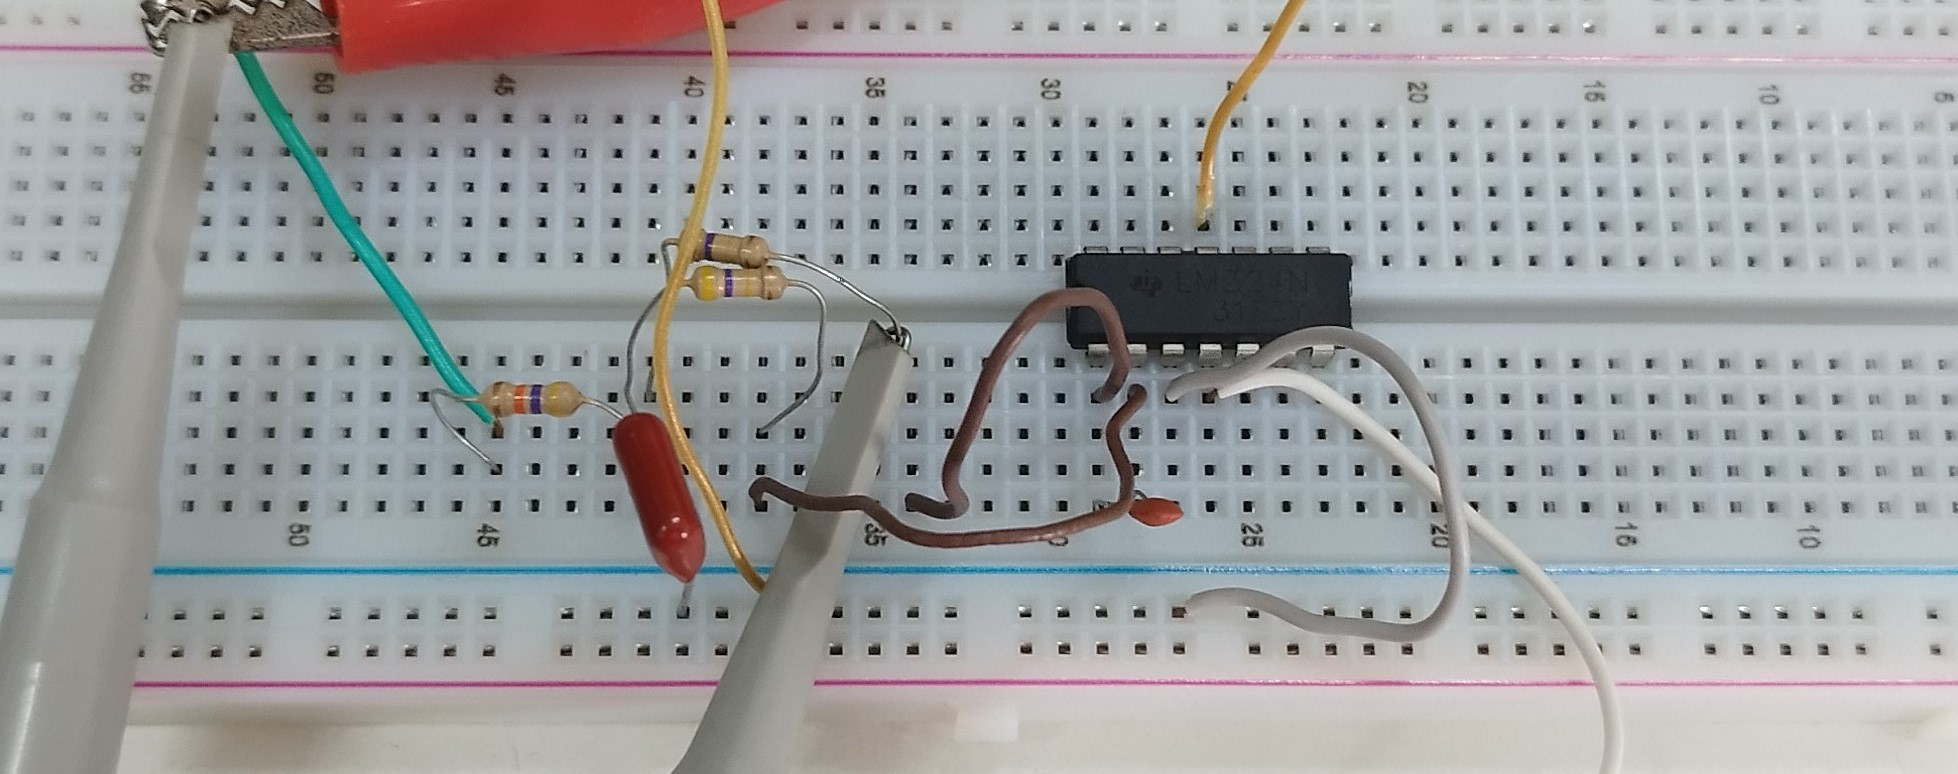
\includegraphics[width=\linewidth]{slides/img/montagem_protoboard.jpg}

      \vspace{0.10cm}
      \scriptsize Montagem em protoboard: acervo da prática.

      \begin{block}{Instrumentação}
        \small Fonte simétrica, multímetro, gerador de sinais e osciloscópio
        para observar entrada e saída.
      \end{block}
    \end{column}
    \begin{column}{0.51\textwidth}
      \centering
      \small
      \textbf{Valores registrados no relatório}

      \vspace{0.12cm}
      \renewcommand{\arraystretch}{1.16}
      \begin{tabular}{lcc}
        \toprule
        Componente & Nominal & Medido \\
        \midrule
        $C_1$ & $100\,\mathrm{nF}$ & $109{,}9\,\mathrm{nF}$ \\
        $C_2$ & $10\,\mathrm{nF}$ & $11{,}42\,\mathrm{nF}$ \\
        $R_1$ & $470\,\mathrm{k}\Omega$ & $469{,}4\,\mathrm{k}\Omega$ \\
        $R_2$ & $470\,\mathrm{k}\Omega$ & $478{,}0\,\mathrm{k}\Omega$ \\
        $R_3$ & $47\,\mathrm{k}\Omega$ & $47{,}13\,\mathrm{k}\Omega$ \\
        \bottomrule
      \end{tabular}

      \vspace{0.16cm}
      \scriptsize A identificação dos resistores nesta tabela corresponde ao
      circuito 2. As curvas teóricas desta apresentação usam os valores nominais.
    \end{column}
  \end{columns}
\end{frame}

\begin{frame}{Amplitudes medidas em bancada}
  \small
  \renewcommand{\arraystretch}{0.93}
  \begin{columns}[T,onlytextwidth]
    \begin{column}{0.48\textwidth}
      \centering
      \textbf{Circuito 1: $V_i=78$--$155\,\mathrm{mV}$}

      \vspace{0.10cm}
      \begin{tabular}{rr}
        \toprule
        $f$ (Hz) & $V_o$ (V) \\
        \midrule
        0,6 & 0,750 \\
        1,7 & 1,050 \\
        2,5 & 0,960 \\
        4,3 & 0,730 \\
        5,2 & 0,640 \\
        6,0 & 0,570 \\
        7,7 & 0,460 \\
        10,8 & 0,340 \\
        17,2 & 0,210 \\
        25,8 & 0,140 \\
        43,0 & 0,060 \\
        \bottomrule
      \end{tabular}
    \end{column}
    \begin{column}{0.48\textwidth}
      \centering
      \textbf{Circuito 2: $V_i=4{,}7$--$5{,}1\,\mathrm{V}$}

      \vspace{0.10cm}
      \begin{tabular}{rr}
        \toprule
        $f$ (Hz) & $V_o$ (V) \\
        \midrule
        2,6 & 4,700 \\
        7,0 & 5,000 \\
        10,5 & 5,100 \\
        17,5 & 5,000 \\
        21,0 & 4,700 \\
        24,5 & 4,600 \\
        31,0 & 3,900 \\
        43,7 & 2,700 \\
        70,0 & 1,300 \\
        105,0 & 0,600 \\
        175,0 & 0,220 \\
        \bottomrule
      \end{tabular}
    \end{column}
  \end{columns}

  \vspace{0.14cm}
  \centering\scriptsize
  Amplitudes de saída convertidas para volts.
  A tensão de entrada foi medida em cada frequência da varredura.
\end{frame}

\begin{frame}{Formas de onda transitórias registradas}
  \small
  \begin{columns}[T,onlytextwidth]
    \begin{column}{0.48\textwidth}
      \centering
      \textbf{Registro com resposta monótona}

      \vspace{0.12cm}
      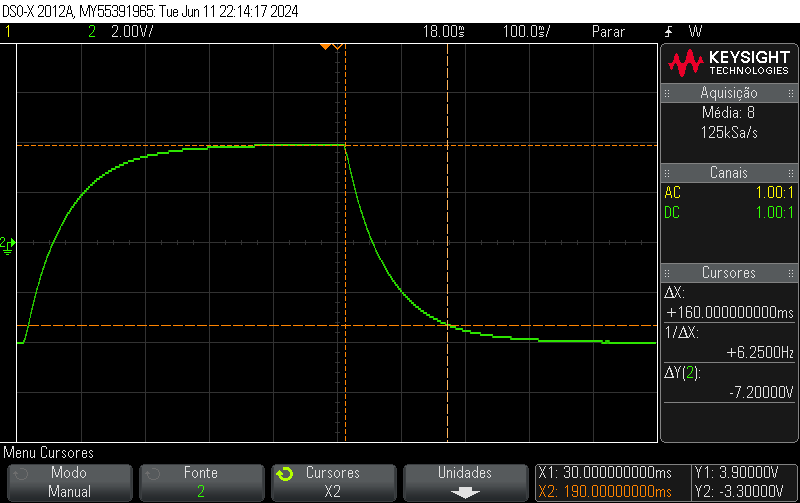
\includegraphics[width=\linewidth,height=0.43\textheight,keepaspectratio]{slides/img/transitorio_monotono.jpg}

      \vspace{0.12cm}
      Cursor em $-7{,}2\,\mathrm{V}$ e $160\,\mathrm{ms}$.\\
      Circuito 1: níveis de $-0{,}8\,\mathrm{V}$ (10\%) e $-7{,}2\,\mathrm{V}$ (90\%).
    \end{column}
    \begin{column}{0.48\textwidth}
      \centering
      \textbf{Registro com oscilação amortecida}

      \vspace{0.12cm}
      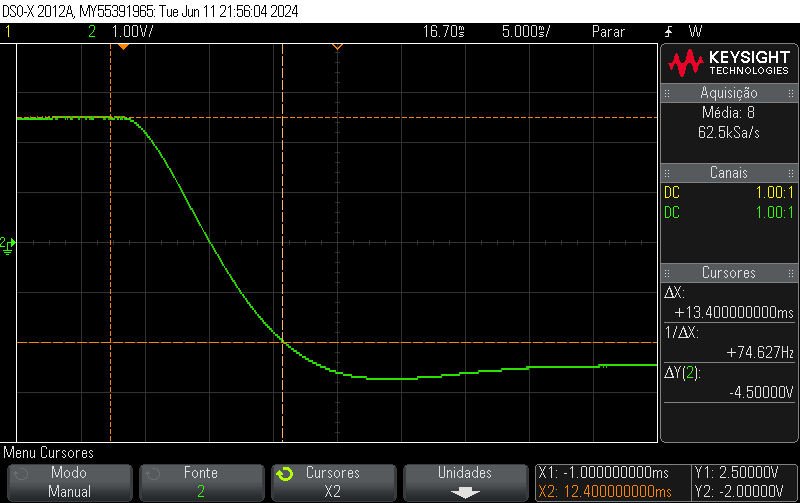
\includegraphics[width=\linewidth,height=0.43\textheight,keepaspectratio]{slides/img/transitorio_oscilatorio.jpg}

      \vspace{0.12cm}
      Cursor em $-4{,}5\,\mathrm{V}$ e $13{,}4\,\mathrm{ms}$.\\
      Circuito 2: níveis de $-0{,}5\,\mathrm{V}$ (10\%) e $-4{,}5\,\mathrm{V}$ (90\%).
    \end{column}
  \end{columns}

  \vspace{0.20cm}
  \centering\scriptsize
  Capturas transitórias preservadas. Os valores finais são $-8\,\mathrm{V}$ no circuito 1
  e $-5\,\mathrm{V}$ no circuito 2; os cursores mostram os registros das imagens.
\end{frame}


\section{Discussão}
\begin{frame}{Comparação entre teoria e experimento}
  \begin{columns}[T,onlytextwidth]
    \begin{column}{0.48\textwidth}
      \centering
      \textbf{Circuito 1}

      \begin{tikzpicture}
        \begin{semilogxaxis}[
          grafico,xmin=0.3,xmax=50,ymin=0,ymax=10.5,
          xlabel={Frequência (Hz)},ylabel={Magnitude $|H|$ (V/V)},
          legend pos=north east
        ]
          \addplot[very thick,RoxoPrincipal] table[x=f,y expr={10^(\thisrow{ganho1_db}/20)}]{slides/dados/resposta_frequencia.dat};
          \addlegendentry{Modelo nominal}
          \addplot[only marks,mark=*,mark size=2pt,MalvaDestaque]
            table[x=f1,y expr={\thisrow{vo1_v}/\thisrow{vi1_v}}]{slides/dados/medicoes_frequencia.dat};
          \addlegendentry{Bancada}
        \end{semilogxaxis}
      \end{tikzpicture}
    \end{column}
    \begin{column}{0.48\textwidth}
      \centering
      \textbf{Circuito 2}

      \begin{tikzpicture}
        \begin{semilogxaxis}[
          grafico,xmin=1,xmax=200,ymin=0,ymax=1.15,
          xlabel={Frequência (Hz)},ylabel={Magnitude $|H|$ (V/V)},
          legend pos=south west
        ]
          \addplot[very thick,RoxoPrincipal] table[x=f,y expr={10^(\thisrow{ganho2_db}/20)}]{slides/dados/resposta_frequencia.dat};
          \addlegendentry{Modelo nominal}
          \addplot[only marks,mark=*,mark size=2pt,MalvaDestaque]
            table[x=f2,y expr={\thisrow{vo2_v}/\thisrow{vi2_v}}]{slides/dados/medicoes_frequencia.dat};
          \addlegendentry{Bancada}
        \end{semilogxaxis}
      \end{tikzpicture}
    \end{column}
  \end{columns}

  \small
  \begin{block}{Comportamentos observados}
    A atenuação do circuito 1 é gradual. No circuito 2, o ganho permanece próximo
    da unidade e a frequência de pico registrada é $17{,}5\,\mathrm{Hz}$.
  \end{block}
  \centering\scriptsize
  Curvas com componentes nominais; pontos calculados por $|H|=V_o/V_i$
  com as tensões de entrada e saída medidas em cada frequência.
\end{frame}

\begin{frame}{Discussão dos resultados e limites dos registros}
  \small
  \centering
  \renewcommand{\arraystretch}{0.98}
  \begin{tabular}{lccc}
    \toprule
    Grandeza & Teoria & Bancada & Diferença relativa \\
    \midrule
    $f_c$ -- circuito 1 & $3{,}03\,\mathrm{Hz}$ & $4{,}3\,\mathrm{Hz}$ & $41{,}9\%$ \\
    $f_{\max}$ -- circuito 2 & $17{,}92\,\mathrm{Hz}$ & $17{,}5\,\mathrm{Hz}$ & $2{,}3\%$ \\
    $t_r$ -- circuito 1 & $115{,}18\,\mathrm{ms}$ & -- & -- \\
    $t_r$ -- circuito 2 & $8{,}71\,\mathrm{ms}$ & -- & -- \\
    \bottomrule
  \end{tabular}

  \vspace{0.05cm}
  {\scriptsize $f_c$ referida ao ganho DC; $t_r=t_{90}-t_{10}$ calculado de $H(s)$.
  Pares experimentais $(t_{10},t_{90})$ não informados.\par}

  \begin{columns}[T,onlytextwidth]
    \begin{column}{0.48\textwidth}
      \begin{block}{Interpretação}
        \begin{itemize}
          \item O corte do circuito 1 apresenta desvio de $41{,}9\%$.
          \item O circuito 2 responde mais rapidamente e apresenta sobressinal.
          \item Tolerâncias e leitura dos cursores podem contribuir para os desvios.
        \end{itemize}
      \end{block}
    \end{column}
    \begin{column}{0.48\textwidth}
      \begin{alertblock}{Valores experimentais}
        \begin{itemize}
          \item Corte do circuito 1: $4{,}3\,\mathrm{Hz}$, com $V_o=730\,\mathrm{mV}$.
          \item Pico registrado no circuito 2: $17{,}5\,\mathrm{Hz}$, com $V_o=5{,}0\,\mathrm{V}$.
          \item A entrada varia na varredura; o ganho é calculado por $V_o/V_i$.
        \end{itemize}
      \end{alertblock}
    \end{column}
  \end{columns}
\end{frame}


\section{Conclusão}
\begin{frame}{Conclusões}
  \begin{itemize}
    \item A função de transferência descreve um filtro ativo passa-baixa de segunda ordem.
    \item A troca de $R_1$ e $R_3$ reduz a magnitude do ganho em DC de 10 para 1
      e altera o circuito de sobreamortecido para subamortecido.
    \item O circuito 1 tende a $-8\,\mathrm{V}$ para o degrau de $0{,}8\,\mathrm{V}$;
      o circuito 2 tende a $-5\,\mathrm{V}$ para o degrau de $5\,\mathrm{V}$.
    \item O LTspice e a bancada reproduzem a atenuação em altas frequências e
      as diferenças entre as configurações.
    \item O corte do circuito 1 foi registrado em $4{,}3\,\mathrm{Hz}$ e o pico do
      circuito 2 em $17{,}5\,\mathrm{Hz}$; os valores teóricos são $3{,}03$ e $17{,}92\,\mathrm{Hz}$.
  \end{itemize}

  \begin{alertblock}{Síntese da prática}
    A posição dos polos conecta o comportamento em frequência ao transitório.
    A comparação experimental considera a variação da tensão de entrada durante
    a varredura, utilizando o ganho $V_o/V_i$ em cada frequência.
  \end{alertblock}
\end{frame}


\section{Referências}
\begingroup
\setbeamertemplate{bibliography item}[text]
\setbeamercolor{bibliography item}{fg=MalvaDestaque}
\setbeamercolor{bibliography entry author}{fg=RoxoPrincipal}
\setbeamercolor{bibliography entry title}{fg=CinzaTexto}
\setbeamercolor{bibliography entry location}{fg=RoxoSecundario}
\setbeamerfont{bibliography entry author}{series=\bfseries}
\setbeamertemplate{bibliography entry title}{\hspace{0.35em}}
\setbeamertemplate{bibliography entry location}{\hspace{0.35em}}
\setbeamertemplate{bibliography entry note}{\hspace{0.35em}}

\begin{frame}[t]{Referências bibliográficas}
  \vspace{0.04cm}
  \fontsize{8.2}{9.3}\selectfont
  \nocite{*}
  \bibliographystyle{plain}
  \bibliography{referencias}
\end{frame}
\endgroup


{
\setbeamercolor{background canvas}{bg=RoxoPrincipal}
\setbeamertemplate{footline}{}
\begin{frame}[plain]
  \begin{center}
    \vfill
    \marcaInstitucional{1.25cm}\par
    \vspace{0.55cm}
    {\color{white}\Huge\bfseries OBRIGADO}\par
    \vspace{0.4cm}
    {\color{MalvaDestaque}\rule{0.22\textwidth}{2pt}}\par
    \vspace{0.55cm}
    {\usebeamerfont{author}\color{white}\insertauthor\par}
    \vspace{0.18cm}
    {\usebeamerfont{institute}\color{white!84}\insertinstitute\par}
    \vspace{0.32cm}
    {\color{MalvaDestaque}\small\bfseries\portfolio\par}
    \vfill
  \end{center}
\end{frame}
}


\end{document}
